%%%% This CV has been greatly influence by
%%%% the extended fancy cv from Carmine Benedetto.
%%%% I thank him for the excellent work. Unfortunately 
%%%% it wouldn't compile on my machine. So I worked it out myself.

\documentclass{article} 
\usepackage[ngerman]{babel}% deutsche Trennregeln
\usepackage{microtype}% verbesserter Randausgleich
\usepackage[utf8]{inputenc}
\usepackage{graphicx}
\usepackage{color}
\usepackage{xcolor}
\usepackage[obeyspaces]{url} 
\usepackage[left=0.5cm,top=0cm,right=0.5cm,bottom=0.2cm,nohead,nofoot]{geometry}

\usepackage{fontawesome}
\usepackage{svg}

\makeatletter
\setlength{\@fptop}{40pt}
\makeatother



\usepackage{pdfcomment}
%% Fix incorrect display of tooltips (http://tex.stackexchange.com/a/74340/3323)
\makeatletter
\renewcommand{\pc@annot@tooltip}%
{%
  /TU (\pc@pdfenc@contents)\space%
  /T (tooltip \thezref@unique)\space%
  /C [0 0 0]\space%
  /FT/Btn\space%
  /Ff 65536\space%
  /H/N\space%
}%

\newcommand{\spacingWork}{0.25cm}

  
\definecolor{white}{RGB}{255,255,255}
\definecolor{anti-flashwhite}{rgb}{0.95, 0.95, 0.96}

\definecolor{darkgray}{HTML}{333333}
\definecolor{gray}{HTML}{4D4D4D}
\definecolor{lightgray}{HTML}{999999}

\definecolor{green}{HTML}{C2E15F}
\definecolor{orange}{HTML}{FDA333}
\definecolor{purple}{HTML}{D3A4F9}
\definecolor{red}{HTML}{FB4485}
\definecolor{blue}{HTML}{6CE0F1}
\definecolor{pblue}{HTML}{0395DE}

\usepackage{tikz}
\newcommand*{\ClipSep}{0.1cm}%


\usetikzlibrary{mindmap,shadows,positioning,backgrounds}

\renewcommand{\thempfootnote}{\arabic{mpfootnote}}

\usepackage{hyperref}
\hypersetup{
    pdftitle={},
    pdfauthor={},
    pdfsubject={},
    pdfkeywords={},
    colorlinks=false,       % no lik border color
   allbordercolors=white    % white border color for all
}

\pagestyle{empty}


%%%%%%%%%%%%%%%%%%%%%%%%%%%%%%%%%%%%%%%%%%%%%%%%%%%%%%%%%%%%%%%%%%%%%%%%%%%%%%%%%%%%%%%%%%%%%%%
\begin{document}
\noindent
\begin{minipage}[t]{0.21\textwidth}
\vspace{0pt}
\centering
\begin{tikzpicture}
			\node [inner sep=0pt] at (0,0) {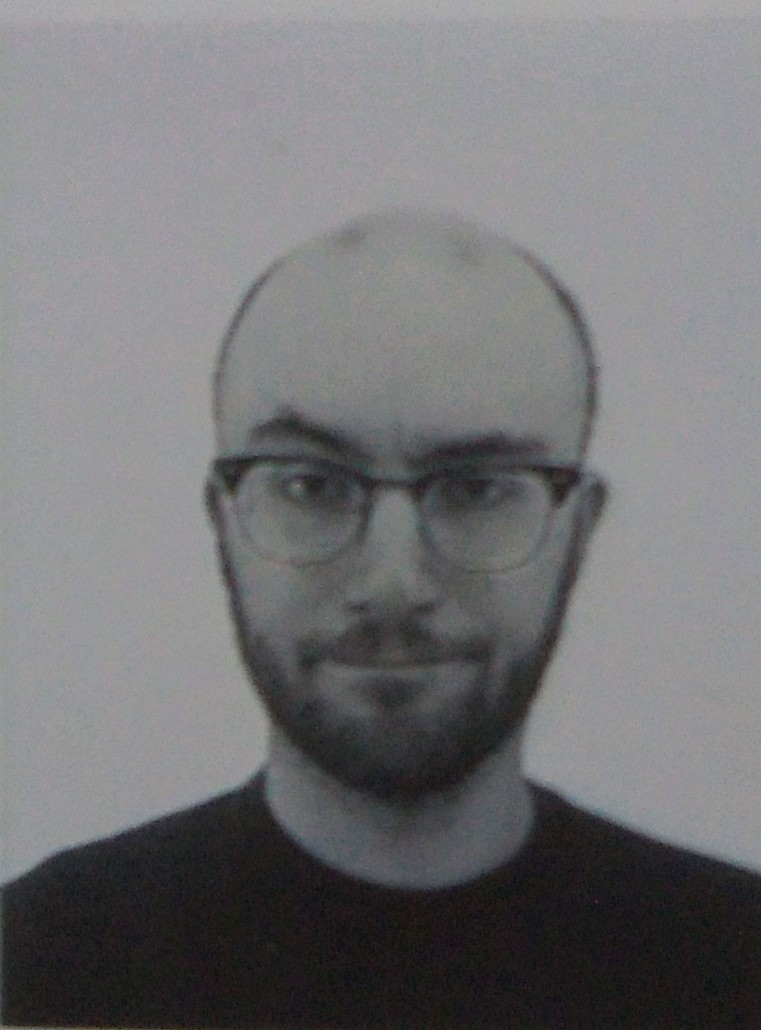
\includegraphics[trim=0cm 1cm 0cm 4cm, clip,scale = 0.12]{../../img/me.jpg}};
			\draw [anti-flashwhite, rounded corners=\ClipSep, line width=\ClipSep]
			(current bounding box.north west) --
			(current bounding box.north east) --
			(current bounding box.south east) --
			(current bounding box.south west) -- cycle
			;
		\end{tikzpicture}
		\faMapMarker~ Potsdam, Deutschland\\

		\vspace{0.15cm}
		{\color{pblue}\faPhone}	+49 174/6507598

		\vspace{0.15cm}
		{\color{pblue}\faEnvelope}~\href{mailto:silvio{\_}schwarz@web.de}{silvio{\_}schwarz@web.de}%\href{mailto:admin@silvioschwarz.com}{admin@silvioschwarz.com}\\
		
		\vspace{0.25cm}
		
		{\Large 
		%\href{https://www.silvioschwarz.com}{\faHome} \hfill 
		\href{https://github.com/silvioschwarz}{\faGithub}  \hfill 
		\href{silvioschwarz.}{\faSkype} 
		\hfill \href{https://www.linkedin.com/in/silvioschwarz/}{\faLinkedin} \hfill 
		\href{https://silvioschwarz.github.io}{\faGithubAlt} \hfill  
		\href{ www.kaggle.com/amethodtomadness/}{
\includegraphics{../../img/kaggle.png}}}
		
%	\section*{\hfill \fontsize{18pt}{24pt}\selectfont \color{pblue} Global Experience}
%	\vspace{-2mm}
%	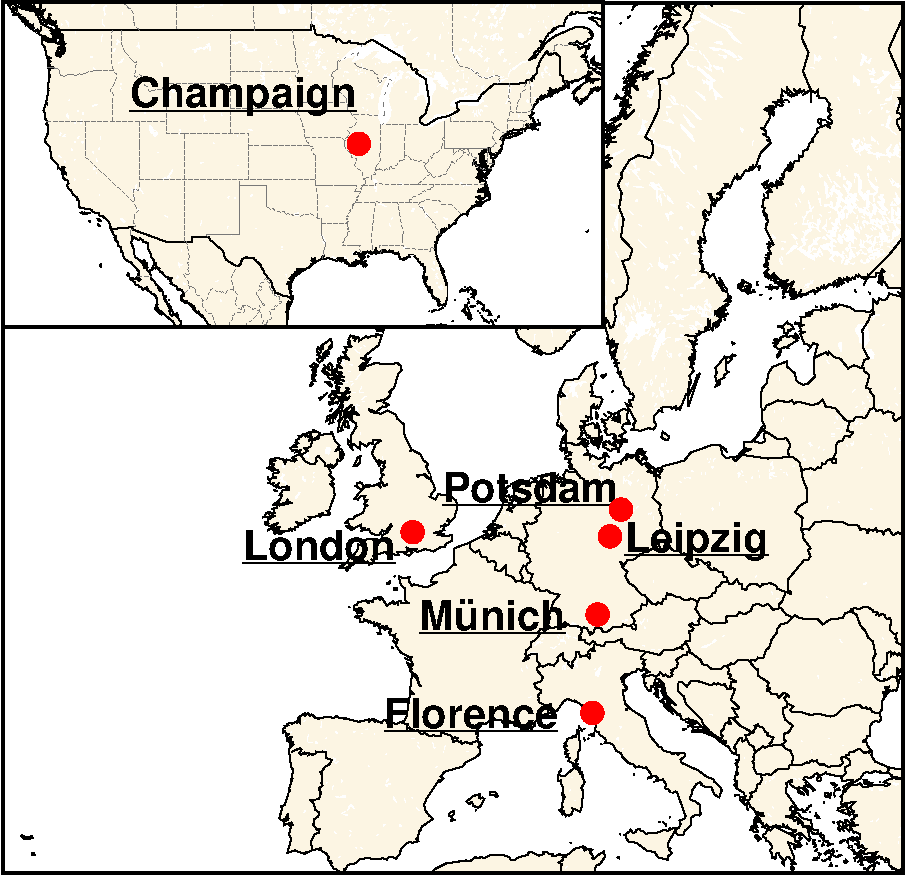
\includegraphics[trim=0cm 0cm 0cm 0cm, clip,scale=0.38]{../../img/globalEXPENG.pdf}
	\vspace{2mm}
	\hrule
	\vspace{-3mm}
	\section*{\fontsize{18pt}{24pt}\selectfont \color{pblue} Programmierung}
	\vspace{0.5mm}
	\textbf{\LARGE \faLinux}
\includegraphics[scale=0.50]{../../img/5stars.png}\\
	\textbf{\LARGE \faWindows}
\includegraphics[scale=0.50]{../../img/3stars.png}\\
	\vspace{5mm}
	
    \begin{tikzpicture}[node distance = 7mm, terminal/.style={
    	rectangle, minimum height = 2mm, rounded corners = 1mm, thick, 
    	draw = darkgray, fill = white, align = left}]
    	\node (A) [terminal] {Python};
    	\node (AA) [terminal, right=2mm of A.east,anchor=west] {R};
    	\node (AAA) [terminal, right=2mm of AA.east,anchor=west] {Matlab};
    	\node (C) [terminal, below=of A.west,anchor=west] {Mathematica};
    	\node (CC) [terminal, right=2mm of C.east,anchor=west] {Latex};
    	\node (D) [terminal, below=of C.west,anchor=west] {HTML/CSS/JS};
    	\node (DD) [terminal, right=2mm of D.east,anchor=west] {ArcGIS};
   		\node (E) [terminal, below=of D.west,anchor=west] {BASH};
    	\node (F) [terminal, right=2mm of E.east,anchor=west] {QGIS};
    	\node (FF) [terminal, right=2mm of F.east,anchor=west] {Git/GitHub};
    	\node (G) [terminal, below=of E.west,anchor=west] {GMT};
	\end{tikzpicture}
	
	\vspace{3mm}
	%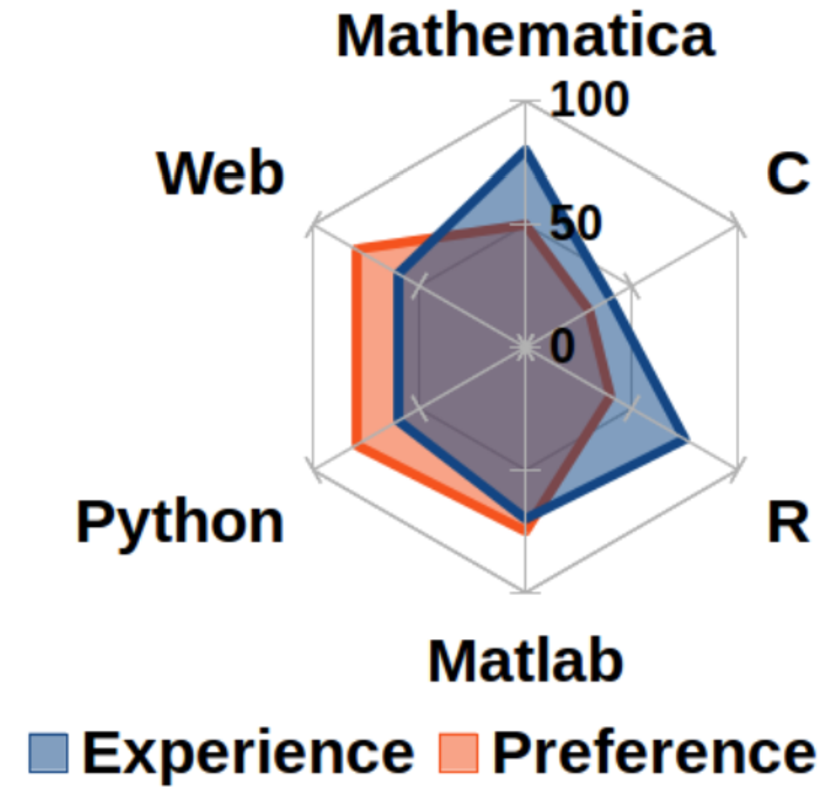
\includegraphics[scale=0.3]{../../img/programming.pdf}
	
	\hrule
	\vspace{-2mm}
	\section*{\fontsize{18pt}{24pt}\selectfont \color{pblue} Sprachen}
	\vspace{-2mm}
	\begin{itemize}
		\raggedleft
		\item[\textbf{Deutsch}] 
\includegraphics[scale=0.50]{../../img/5stars.png}\vspace{-2mm}
		\item[\textbf{Englisch}]  
\includegraphics[scale=0.50]{../../img/5stars.png}\vspace{-2mm}
		\item[\textbf{Italienisch}] 
\includegraphics[scale=0.5]{../../img/3stars.png}\vspace{-2mm}
		\item[\textbf{Französisch}]  
\includegraphics[scale=0.50]{../../img/2stars.png}
	\end{itemize}
	\hrule
	\vspace{-2mm}
	\section*{\fontsize{18pt}{24pt}\selectfont \color{pblue} Kenntnisse}
	\vspace{0.5mm}
    \begin{tikzpicture}[node distance = 7mm, terminal/.style={
    	rectangle, minimum height = 2mm, rounded corners = 1mm, thick, 
    	draw = darkgray, fill = white, align = left}]
    	\node (A) [terminal] {seismische Gefährdungsanalyse};
    	\node (AA) [terminal, below=of A.west,anchor=west] {IoT};
    	\node (B) [terminal, right=2mm of AA.east,anchor=west] {Bodenbewegungsmodelle};
    	\node (AAA) [terminal,  below=of AA.west,anchor=west] {maschinelles Lernen};
    	\node (AAAA) [terminal,  below=of AAA.west,anchor=west] {Bayesische Statistik};
    	\node (C) [terminal,  below=of AAAA.west,anchor=west] {interaktive Visualisierung};
	\end{tikzpicture}
	\vspace{2mm}
	\hrule
	\vspace{-2mm}
	\section*{\fontsize{18pt}{24pt}\selectfont \color{pblue} Interessen}
	\vspace{-2mm}
	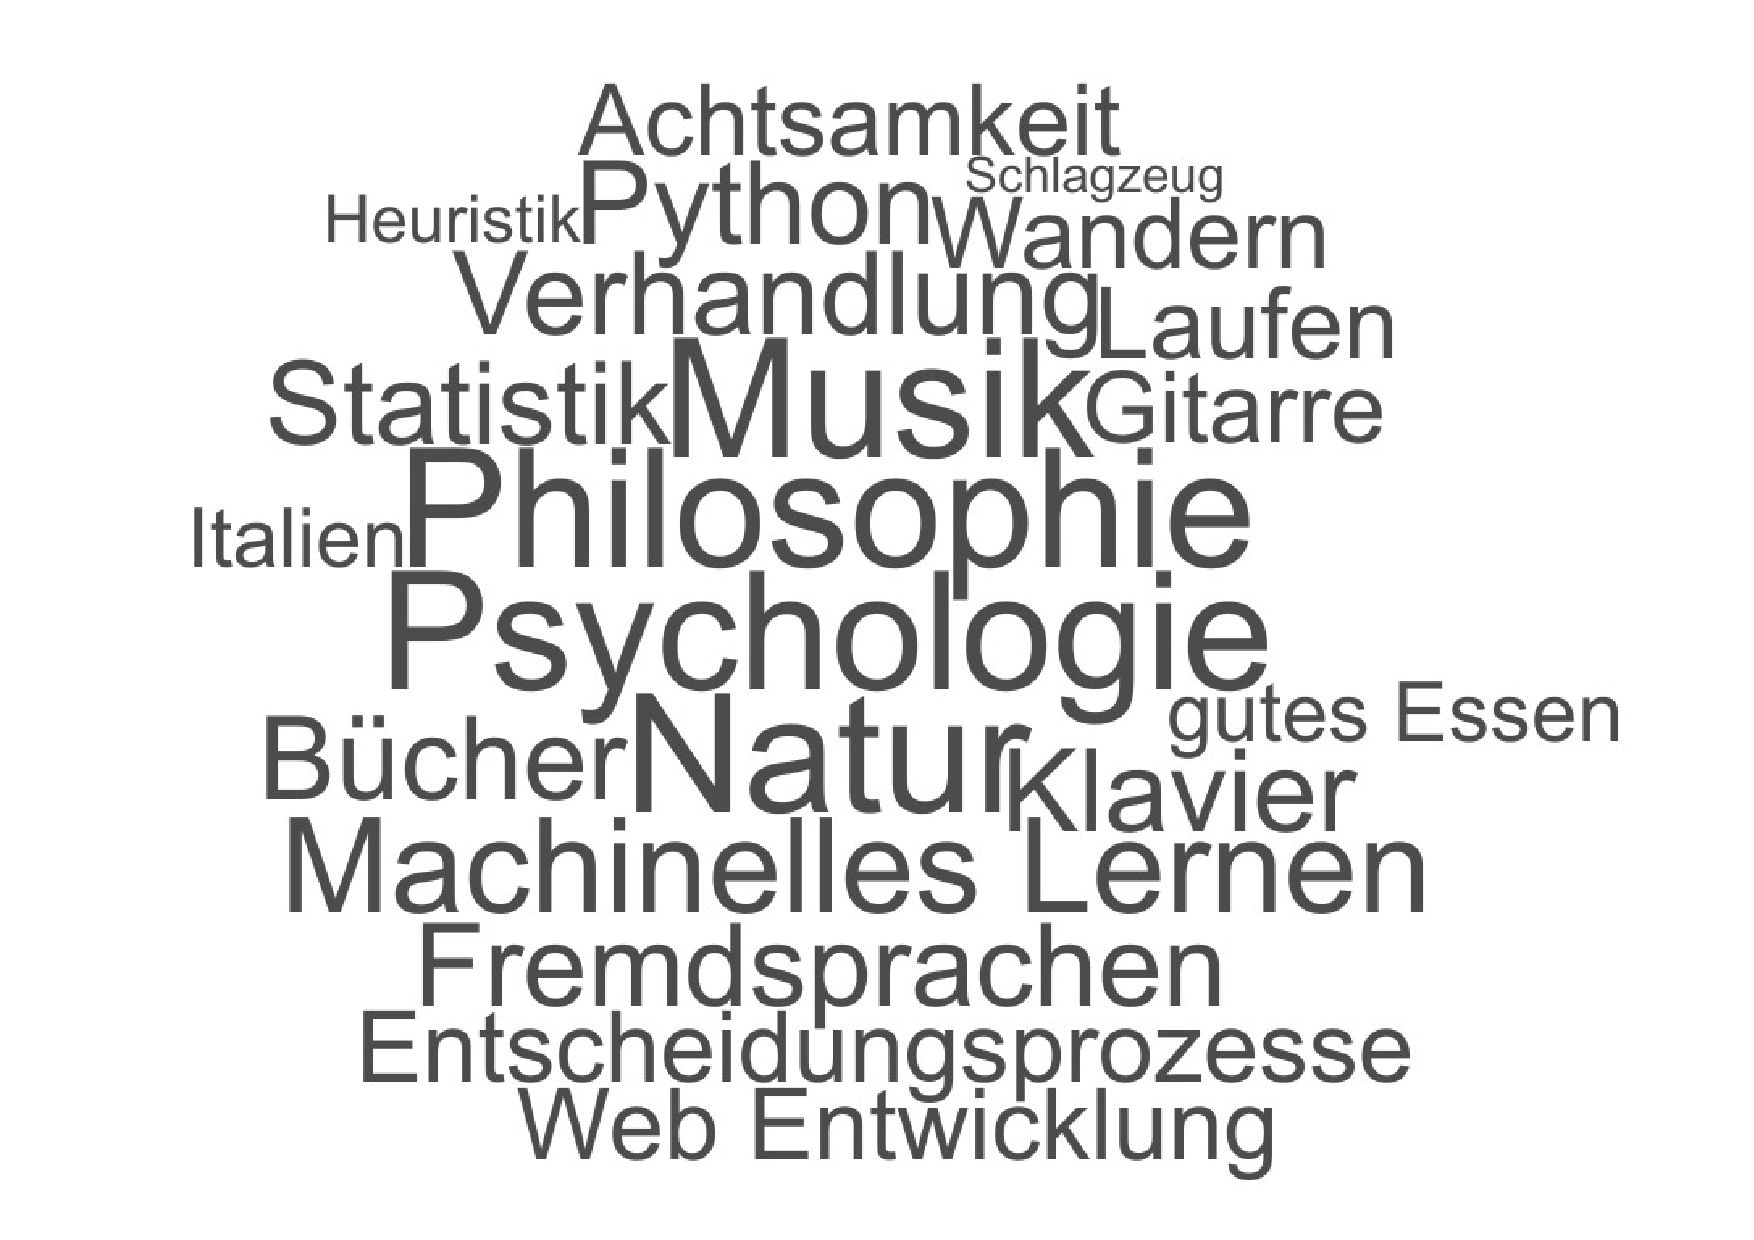
\includegraphics[trim=3cm 1cm 2cm 1cm, clip,scale=0.21]{../../img/wordcloudGER.pdf}
\end{minipage}
%%%%%%%%%%%%%%%%%%%%%%%%%%%%%%%%%%%%%%%%%%%%%%%%%%%%%%%%%%%%%%%%%%%%%%%%%%%%%%%%%%%%%%%%%%%%%%%%%%%
\hfill
\vrule
\hfill
\begin{minipage}[t]{0.69\textwidth}
\vspace{0pt}
%	\begin{minipage}[t]{0.49\textwidth}
	{\fontsize{30pt}{62pt}\color{gray} \selectfont {Silvio}{\textbf{Schwarz}}}\\
	{\fontsize{14pt}{24pt}\color{pblue} \selectfont Geowissenschaftler \color{lightgray} (B.Sc.)}\\
	\hrule
	\section*{\fontsize{18pt}{24pt}\selectfont \color{pblue} Bildung}
	\begin{minipage}[t]{0.2\textwidth}
			\centering
			10/2011 - 10/2019\\(8 Jahre)
		\end{minipage}
		\hfill
		\begin{minipage}[t]{0.75\textwidth}
		\textbf{\color{pblue}\faHourglassHalf~Master of Science}\footnote{\label{1} auf Grund von Krankheit abgebrochen}\hfill
		\href{https://www.uni-potsdam.de/}{\color{pblue}Universität Potsdam} \\
		\textbf{\underline{Geowissenschaften}}\\
		\textbf{\underline{Vertiefung:}~Geophysik, Seismologie, maschinelles Lernen}\\
		\textbf{\underline{Abschlussarbeit}}:\\ 1) \href{https://github.com/silvioschwarz/master-thesis}{Forecasting Macroseismic Intensities: A Sensitivity Study of a Bayesian Approach\textsuperscript{\ref{1}} 2014-2016} \\
		2) Classification of eruptive tremor sources during the 2014-2015 Holuhraun sequence, Iceland\textsuperscript{\ref{1}} 2019
	\end{minipage}\\\\\\
	\hfill
	\begin{minipage}[t]{0.2\textwidth}
			\centering
			10/2008 - 09/2011\\(3 Jahre)
		\end{minipage}
		\hfill
		\begin{minipage}[t]{0.75\textwidth}
		\textbf{\href{https://www.dropbox.com/s/297g1chiby8mrd3/Bachelor-Certificate.pdf?dl=0}{\color{pblue}\faGraduationCap~Bachelor of Science}} \hfill	\href{https://www.uni-potsdam.de/}{\color{pblue}Universität Potsdam}\\
		\textbf{\underline{Geowissenschaften}}\\
		\textbf{Geologie, Physik, Mathematik, Chemie}\\
		\textbf{\underline{Abschlussarbeit}}:
		 \href{https://www.dropbox.com/s/3kngo4hpb0c47ww/Bachelorarbeit.pdf?dl=0}{\pdftooltip{Simulation von Bodenbewegungsszenarien von Starkbeben}{engl.: Simulating Ground Motion Scenarios of strong Earthquakes}} \\	
		\end{minipage}
	\hfill
	\begin{minipage}[t]{0.2\textwidth}
			\centering
			08/2000 - 05/2008\\(8 Jahre)
		\end{minipage}
		\hfill
		\begin{minipage}[t]{0.75\textwidth}
		\textbf{\href{https://www.dropbox.com/s/nsgmvy7o64xb9si/Abiturzeugnis.pdf?dl=0}{\color{pblue}\faGraduationCap~Abitur \hfill \href{https://www.klosterschule.de/}}}{\color{pblue}Klosterschule Roßleben (staatl. Gymnasium)}\\
		\textbf{\underline{Leistungsfächer}}: \textbf{Mathematik}, \textbf{Geographie}\\
		\textbf{\underline{Seminarfacharbeit}}:
		\pdftooltip{Naturkatastrophen und ihr Einfluss auf das Leben in der Gegenwart (German)}{engl.: Natural Disasters and their Impact on Life in the Present}
	\end{minipage}\\\\
	\hrule
	%%%%%%%%%%%%%%%%%%%%%%%%%%%%%%%%%%%%%%%%%%%%%%%%%%%%%%%%%%%%%%%%%%%%%%%%%%%%%%%%%
\section*{\fontsize{18pt}{24pt}\selectfont \color{pblue} Erfahrung}
	\begin{minipage}[t]{0.99\textwidth} 
%		\begin{minipage}[t]{0.2\textwidth}
%			\centering
%			11/2017 - 03/2018\\(5 Monats)
%		\end{minipage}
%		\hfill
%		\begin{minipage}[t]{0.75\textwidth}
%			\textbf{Student Trainee}\hfill \href{https://assecor.de/}{\color{pblue}DB Dialog}\\
%			support passenger rights
%		\end{minipage}
%
%		\vspace{\spacingWork}
%

				\begin{minipage}[t]{0.2\textwidth}
				\centering
				05/2019 - 10/2019 \\(6 Monate)
				\end{minipage}
				\hfill
				\begin{minipage}[t]{0.75\textwidth}
				\textbf{Studentische Hilfskraft}\hfill 
				\href{https://www.geo.uni-potsdam.de/}{\color{pblue}Universität Potsdam}\\
				\href{http://www.geo.uni-potsdam.de/allgemeine-geophysik-1570.html}{Arbeitsgruppe Allgemeine Geophysik}\\
			    Characterizing tremor sources during the Holuhraun eruption, Iceland\\
			    \textbf{\underline{Betreuer}}: \href{mailto:eva.eibl@un-potsdam.de }{\color{pblue}Prof. Dr. Eva Eibl }
				\end{minipage} 
				
%		\vspace{\spacingWork}
%		
%				\begin{minipage}[t]{0.25\textwidth}
%				\centering
%				01/2013\\ -\\ 04/2013 \\(3 Monate)
%				\end{minipage}
%				\hfill
%				\begin{minipage}[t]{0.75\textwidth}
%				\textbf{Internship}\footnote{cancelled due to illness}\hfill	
%				\href{https:///www.munichre.com/}{\color{pblue}Munich Re}\\
%				Improvement of GMPE\\
%				\textbf{\underline{Betreuer}}: \href{mailto:MKaeser@munichre.com}{\color{pblue}Prof. Dr. Martin Käser}%https://www.geophysik.uni-muenchen.de/Members/kaeser/cv
%				\end{minipage}
				
		\vspace{\spacingWork}
		
		\begin{minipage}[t]{0.2\textwidth}
			\centering
			08/2014 - 06/2015\\(11 Monate)
		\end{minipage}
		\hfill
		\begin{minipage}[t]{0.75\textwidth}
			\textbf{Werksstudent}\hfill
			\href{https://assecor.de/}{\color{pblue}Assecor GmbH, Berlin, Ger}\\
			Dokumentation des Berliner Stromnetzes in einem Netzinformationssystem für Vattenfall Europe Sales GmbH
		\end{minipage}

		\vspace{\spacingWork}

		\begin{minipage}[t]{0.2\textwidth}
			\centering
			11/2013 - 03/2014 \\(5 Monate)
		\end{minipage}
		\hfill
		\begin{minipage}[t]{0.75\textwidth}
			\textbf{Werksstudent}\hfill \href{https://assecor.de/}{\color{pblue}Assecor GmbH, Berlin, Ger}\\
			Migration der IT Infrastruktur für BIOTRONIK SE \& Co. KG
		\end{minipage}
		
		\vspace{\spacingWork}
		
				\begin{minipage}[t]{0.2\textwidth}
				\centering
				09/2012 - 11/2012 \\(3 Monate)
				\end{minipage}
				\hfill
				\begin{minipage}[t]{0.75\textwidth}
				\textbf{Master Praktikum}\hfill	
				\href{https:///www.wolframalpha.com/}{\color{pblue}Wolfram$\mid$Alpha, Illinois, USA}\\
				Entwicklung von geophysikalischen Inhalt für Wolfram$~\mid~$Alpha\hfill \href{https://m.wolframalpha.com/input/?i=moment+magnitude}{\color{pblue}Beispiel}\\
				\textbf{\underline{Betreuer}}: \href{mailto:bjornz@wolfram.com }{\color{pblue}Dr. Björn Zimmermann} \&	\href{mailto:mtrott@wolfram.com }{\color{pblue} Dr. Michael Trott}
				\end{minipage}
				
		\vspace{\spacingWork}
		
				\begin{minipage}[t]{0.2\textwidth}
				\centering
				06/2011 - 08/2012 \\(1 Jahr 3 Monate)
				\end{minipage}
				\hfill
				\begin{minipage}[t]{0.75\textwidth}
				\textbf{Studentische Hilfskraft}\hfill		
				\href{https://www.uni-potsdam.de/}{\color{pblue}Universität Potsdam}\\
				SSHAC LEVEL 3 PSHA Modellerstellung und Beratung\\
				1-wöchige Beratung für \href{https://www.imperial.ac.uk/people/j.bommer}{\color{pblue}Prof. Julian J. Bommer}, Imperial College London\\
				\textbf{\underline{Betreuer}:} \href{http://www.geo.uni-potsdam.de/mitarbeiterdetails/show/96/Frank_Scherbaum.html/}{\color{pblue}Prof. Frank Scherbaum}				
				\end{minipage}
				
		\vspace{\spacingWork}
		
				\begin{minipage}[t]{0.2\textwidth}
				\centering
				03/2011 -  04/2011\\(1 Monat)
				\end{minipage}
				\hfill
				\begin{minipage}[t]{0.75\textwidth}
				\textbf{Bachelor Praktikum}\hfill
				\href{http://geologie.physgeo.uni-leipzig.de}{\color{pblue}Universität Leipzig}\\
				Pflege des seismologischen Netzwerkes von Sachsen\\
				\textbf{\underline{Betreuer}}: \href{mailto:sfunke@rz.uni-leipzig.de}{\color{pblue}Dipl. Geophys. S. Funke}
			\end{minipage}		
	\end{minipage}
	\vspace{\spacingWork}
		\hrule
		
		\section*{\fontsize{18pt}{24pt}\selectfont \color{pblue} Projekte}

%		\begin{minipage}[t]{0.2\textwidth}
%			\centering
			\textbf{\large\color{pblue}\href{https://earthquake-distances.herokuapp.com}{EQDist}}\\
%		\end{minipage}
%		\hfill
%		\begin{minipage}[t]{0.75\textwidth}
		{Berechnung und interaktive Visualisierung von Entfernungsmetriken relevant für Bodenbewegungsmodelle}\\\\
%		\end{minipage}
%		
%		\vspace{\spacingWork}
%		
%		\begin{minipage}[t]{0.2\textwidth}
%			\centering
%			\textbf{\large\color{pblue}\href{https://silvioschwarz.github.io/TerremotoPi/}{TerremotoPi}}\\
%		\end{minipage}
%		\hfill
%		\begin{minipage}[t]{0.75\textwidth}
%		{A RaspberryPi powered seismic station with real-time capabilities}\\
%		\end{minipage}
%		
%		\vspace{\spacingWork}
%		
%		\begin{minipage}[t]{0.2\textwidth}
%			\centering
			\textbf{\large\color{pblue}\href{https://terrorxafrica.herokuapp.com}{TerrorXAfrica}}\\
%		\end{minipage}
%		\hfill
%		\begin{minipage}[t]{0.75\textwidth}
		{interaktive Visualisierung bewaffneter Konflikte in Afrika im Rahmen des 22-stündigen Hackathon interactive \href{https://hackhpi2019.devpost.com}{\color{pblue}HackHPI2019} für die IBM cross-border effects challenge}
%		\end{minipage}
%		\begin{itemize}
%		\item TerrorXAfrica
%		\item TerremotoPi \href{https://github.com/silvioschwarz/TerremotoPi}{}
%		\item Eatrhquake source-to-site distances \href{https://github.com/silvioschwarz/Earthquake-Distances}{\faGithub}
%		\end{itemize}
\end{minipage}


\end{document}